\subsection{修改截面视图样式}

由于视图均按标准位置进行配置,且视图绘制比例是一致的,因此不需要标注剖视图的比例,故需要设置截面视图样式。截面视图样式管理器,其启动方法有:
\begin{itemize}
\item 键盘输入 viewsectionstyle\index{viewsectionstyle,截面视图样式}。
\item 【布局】选项卡中的【截面视图样式】图标
\includegraphics[scale=0.6]{viewsectionstyle.png}。
\end{itemize}
启动完成后会出现图\ref{fig:viewsectionstyle5} 所示的截面视图样式管理器对话框。
\clearpage
\begin{figure}[htbp]
\centering
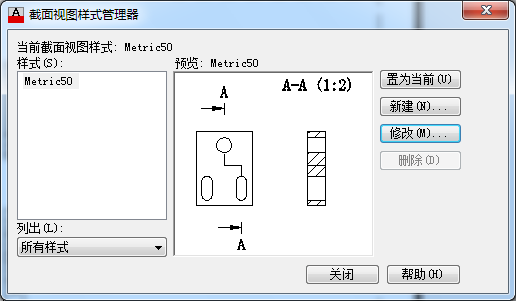
\includegraphics[scale=0.8]{viewsectionstyle5.png}
\caption{截面视图样式管理器对话框}\label{fig:viewsectionstyle5}
\end{figure}

在截面视图样式管理器对话框的样式列表框中选择Metric50,点击修改按钮,弹出图\ref{fig:viewsectionstyle1}所示的对话框,然后选中标识符和箭头选项卡。
\begin{figure}[htbp]
\centering
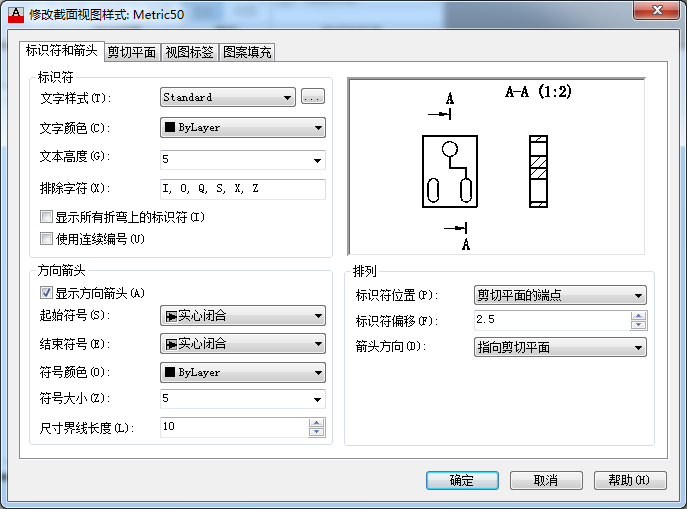
\includegraphics[scale=0.6]{viewsectionstyle1.png}
\caption{标识符和箭头设置}\label{fig:viewsectionstyle1}
\end{figure}

该选项卡中标识符选项组是用于设置截面视图中的剖切标识符的样式;方向箭头选项组用于设置方向箭头的样式;排列选项组用于设置剖切标识符和方向箭头的排列方。根据国家制图标准将排列选项组中的箭头方向修改为“远离剪平面”。

选择剪切平面选项卡,如图\ref{fig:viewsectionstyle2}所示。该选项卡用于设置剪切平面的样式。该选项卡中的端线和折弯线选项组用于设置端线的显示和样式;剖切平面线选项组用于设置剖切平面线的显示和样式。
\begin{figure}[htbp]
\centering
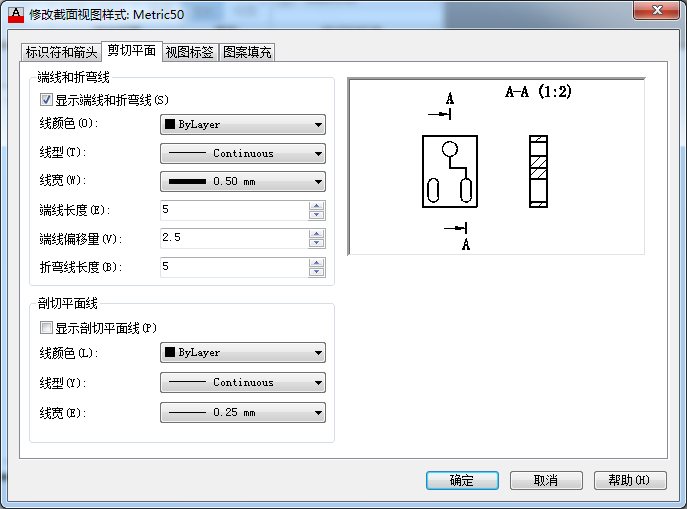
\includegraphics[scale=0.5]{viewsectionstyle2.png}
\caption{剪切平面设置}\label{fig:viewsectionstyle2}
\end{figure}

选择视图标签选项卡,如图\ref{fig:viewsectionstyle3}所示。该选项卡中标签选项组用于设置视图标签是否显示以及显示的样式;标签内容用于设置显示的标签由哪此内容构成。由于整个视图比较是一致的,所以根据国家标准将标签内容中的比例部分删除。
\begin{figure}[htbp]
\centering
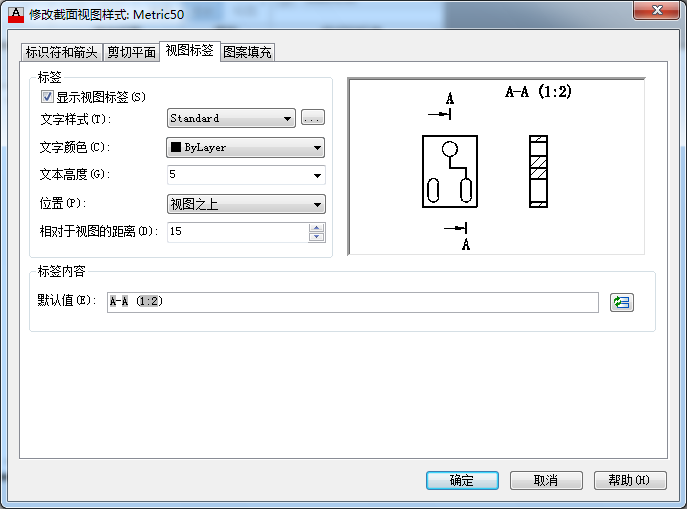
\includegraphics[scale=0.5]{viewsectionstyle3.png}
\caption{视图标签设置}\label{fig:viewsectionstyle3}
\end{figure}

选择图案填充选项卡,如图\ref{fig:viewsectionstyle4}所示。该选项卡主要用于设置填充的剖面线样式。
\clearpage
\begin{figure}[htbp]
\centering
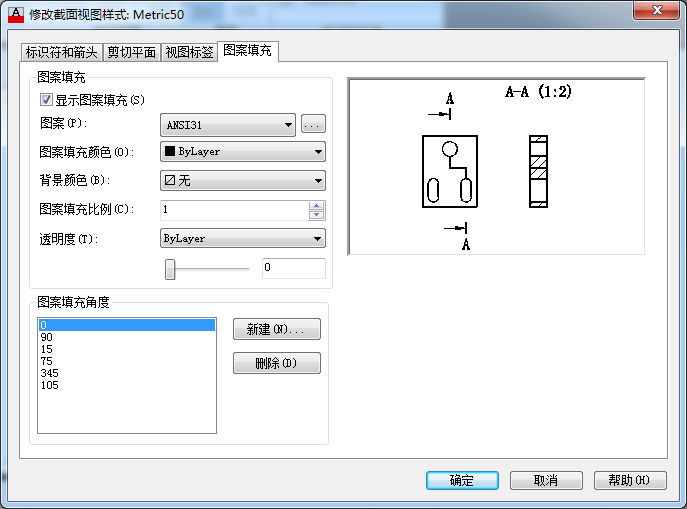
\includegraphics[scale=0.55]{viewsectionstyle4.png}
\caption{图案填充设置}\label{fig:viewsectionstyle4}
\end{figure}

经过上述操作,即可完成截面视图样式的修改,完成后点击确定按钮,最后关闭截面视图样式管理器对话框。修改完成后阀体的三视图布局结果如图\ref{fig:viewsectionstyle6}所示。
\begin{figure}[htbp]
\centering
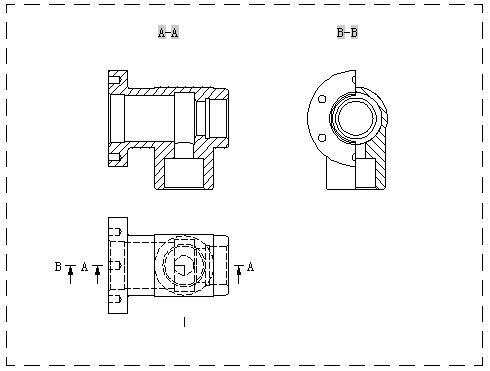
\includegraphics[scale=0.7]{viewsectionstyle6.png}
\caption{阀体三视图布局}\label{fig:viewsectionstyle6}
\end{figure}
\endinput

